\section{Problem and Significance}
The biggest problem of AI is not anymore its perceived usefulness, as this has mostly been solved by its recent successes, but its capacity to elicit the trust of users.
An automated system should be able to make itself be trusted in a manner proportional to the criticality of its application \citep{gilpin2018explaining}, \citep{abdul2018trends}.
The lack of trust that a person may feel, stems from the difficulty in verifying the system's outputs; if no rationale can be inferred for why a given ML model made a certain decision, there is also no way to understand if these outputs conform to our moral norms\footnote{See \citet{gilpin2018explaining} and \citet{abdul2018trends} for a discussion on trust in AI}.
As discussed in Section \ref{sec:importance-of-explainability}, no explicit justification for the link between the explainability and the \textit{trustability} of a model has been found in the reviewed literature; nonetheless, it seems quite natural to infer that a person would not trust decisions made on an unknown rationale. 
Unfortunately, the \textit{explainability} and performance of machine learning models is usually inversely proportional, as is shown in Figure \ref{fig:darpa-comparison-methods}.

There are many examples of modern methods - such as boosted trees, random forests, bagged trees, kernelized-SVMs - that show the tendency outlined in Figure \ref{fig:darpa-comparison-methods}, but this is best exemplified by \textit{deep neural networks} (DNNs). 
Deep Neural Networks are machine learning models constructed by stacking many layers of artificial neurons; these systems are currently offer state of the art performance on a variety of tasks but are among the least easily interpretable systems due to the fact that they represent information in an implicit and distributed manner.  
Some older methods, like decision trees or rule-based methods, are inherently more interpretable due to their simplicity and the fact that they can explicit state their reasoning steps, but are less accurate and flexible than more modern techniques \citep{Biran2017} (as exemplified in Figure \ref{fig:darpa-comparison-methods}).

\begin{figure}[htbp]
\centerline{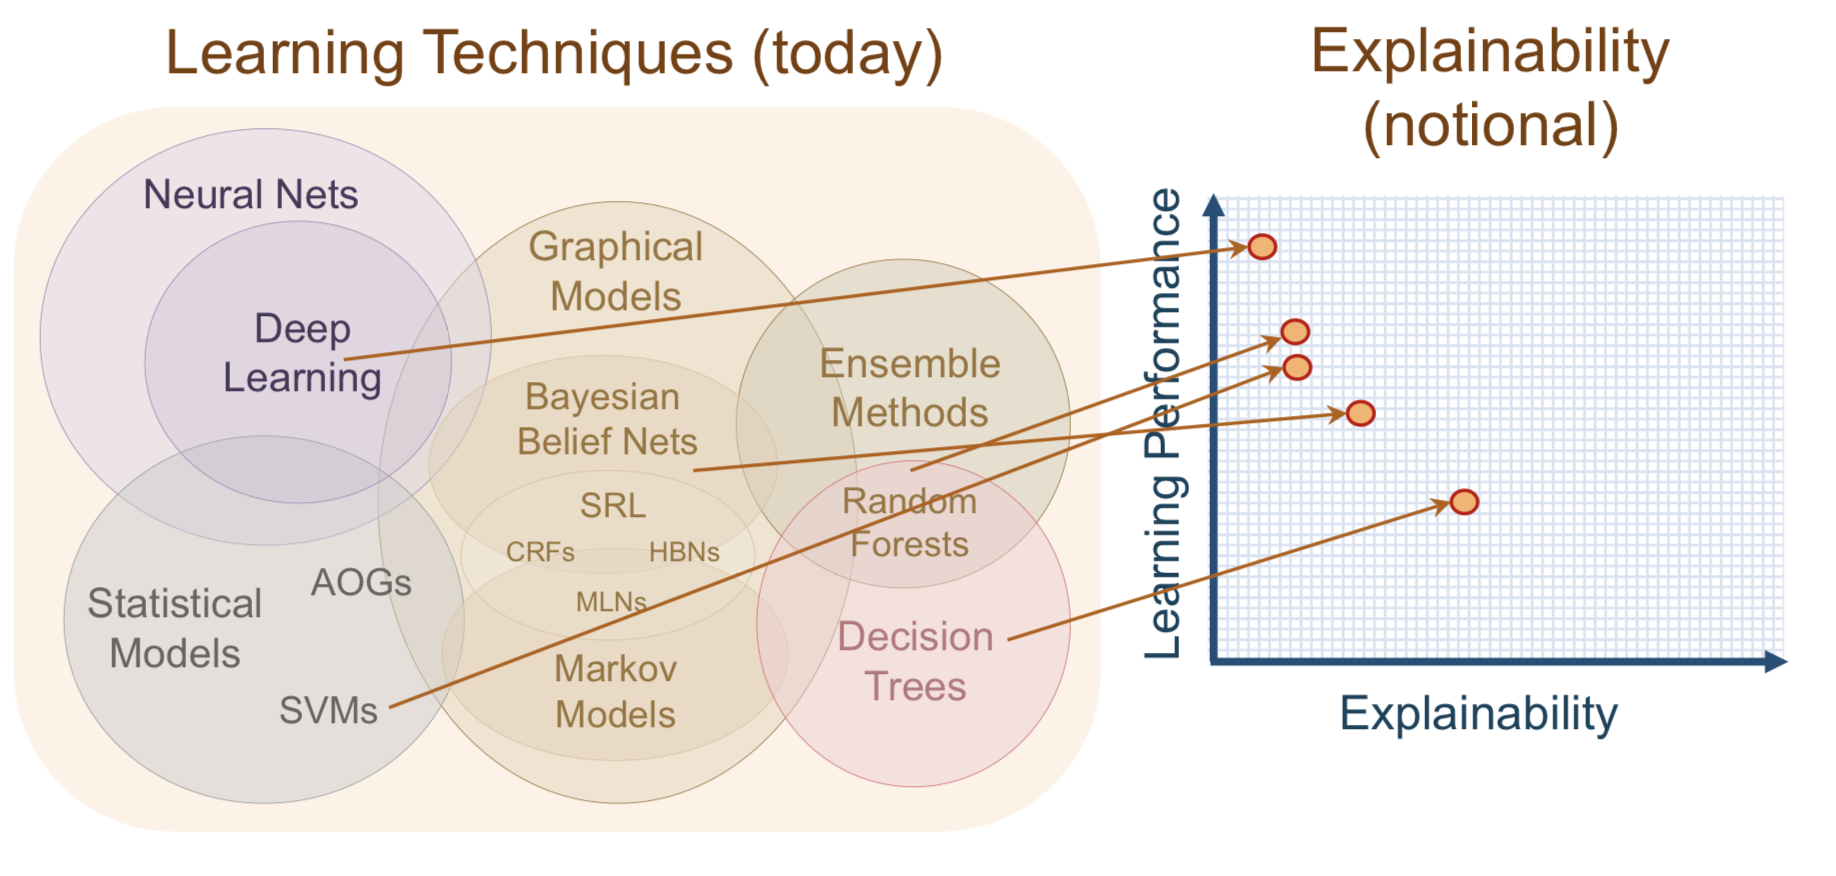
\includegraphics[width=\textwidth]{introduction/images/darpa-comparison-methods}}
\caption{Mapping showing the tradeoff between performance and interpretability of contemporary and older machine learning models \citep{gunning2017explainable}}
\label{fig:darpa-comparison-methods}
\end{figure}

The runaway success obtained by modern Machine Learning in a variety of domains, on a spectrum that goes from engineering to social work, has created the desire to also start applying these methods to mission-critical and traditionally more entrenched fields  (for an overview of deep neural networks as applied to medicine see \citet{Travers2018}).  
A perfect example of an area exhibiting both these characteristics is that of medicine.  
The first successful artificially intelligent systems date back to the 1970s and '80s and were based on \textit{symbolic methods} integrated with \textit{knowledge-bases}.  
These systems were by design capable of providing an explanation for their reasoning and were thus accepted by the medical community in an implementation known as \textit{expert systems}, that aimed to aid in the diagnosis of disease\footnote{For an overview of expert systems see \citet{Liao2005}}. 
The deficiency of modern AI methods in being able to provide causal links for their reasoning process has held back their acceptance in the field of medicine, regardless of their superior performance and accuracy.

One modern ML model that has seen success in the medical domain is that of \textit{Bayesian Networks} (BNs) (defined in much greater detail in Section \ref{sec:bayesiannetworks}), a graphical and computationally efficient way of representing dependencies between variables of interest\footnote{For an overview of BNs in the medical domain see \citet{Lucas2001}}.  
The graphical component is given by the fact that each variable is represented by a node of a Directed Acyclic Graph (DAG) (Definition \ref{def:dag}), with the edges connecting them modelling their dependencies.  
The efficiency stems from the fact that the graph structure imposes a factorisation of the joint probability space and thus lets each variable's values be calculated using only those of its parents.
As is discussed in detail in Section \ref{sec:explainability-in-bayesian-networks}, Bayesian Networks may be uniquely suited to providing effective explanations, by virtue of their inherent characteristics.

In a high-stakes domain such as the medical one, it would be unthinkable for a doctor to trust the predictions of an AI system a priori.
Any decision with profound moral implications - such as prescribing or interrupting the treatment of a patient - would have to first be validated by a human; but, to be able to do so, the clinician would need to be able to understand the rationale behind the machine's output. 
The feasibility of carrying out this validation is dependent on the degree of interpretability of the model that made the decision and, unfortunately, this is the main gap identified in xAI methods.
BNs are no exception, as noted by \cite{timmer2015explaining}, because the underlying formalism makes them appear akin to \enquote{black-boxes} to domain experts who are also not well-versed in statistical reasoning.
Obviously, we don't expect our doctors to also be machine learning experts so the onus of making these models understandable and usable by domain experts falls squarely onto the researchers in the xAI community.
Through a process of real-world validation and testing, they should strive to develop methods that are not only provably correct but, just as importantly, capable of relating efficiently to its intended users.

Explainability is not a necessary condition only for the verification of the system's outputs which, as has just been discussed, is a presupposition for it to be applied in mission-critical domains, but also for the extraction of knowledge from data. 
The amount of information that a machine can process is many orders of magnitude greater than that inspectable by any human; this may let a computer spot new patterns in the data that result undetectable when observing only a moderate amount of samples.   
Being able to understand the mapping from the model's inputs to its outputs, can be seen as understanding the system's \enquote{reasoning} process and could thus lead to knew insights or to the confirmation of existing theories.
This is because understanding the process the model uses to give a certain output can make the machine's analytical power leverageable by our more general/horizontal, but less capable of deep/vertical analysis, capacities.
This is also noted \textit{en passant} by \citet{doshi2017towards} when they state \enquote{humans' goal is to gain knowledge. We do not have a complete way of stating what knowledge is; \textit{thus the best we can do is ask for explanations we can convert into knowledge}}.

In light of all that has been said - that will be explored and justified in much more depth during Chapter \ref{chap:literature-review} - the main focus of this thesis aims to be to address one of the most severe gaps in the current xAI literature: the lack of validation of machine learning systems with real users in real situations.
The work will focus in particular on the medical area and will attempt to evaluate the effectiveness of a Bayesian Network-based system, by an evaluation carried out in collaboration with expert clinical pathologists in a real work setting, over a period of time.
The hope is to validate the current hypothesis that states that Bayesian Networks are inherently apt to being made explainable and also to lay the methodological groundwork for future research aimed at addressing the identified lack of available evaluation in the xAI literature.